
\chapter{The Top Physics and Machine Learning}

\section{The Top Physics}

Top quark, the most massive fundamental particle in Standard Model(SM), is the only quark that decays semi-weakly. Its large mass leads to a short lifetime and decay before hadronization occurs. Top quark contains so many properties that interest us, such as its mass, couplings, and cross-section, e.t.c. Measure these properties accurately can bring us a worth understanding of fundamental interactions and the key to Beyond Standard Model.\cite{Zyla:2020zbs}
\\
In recent model, Top quark pair produced by $pp$ collision has three decay modes, \textbf{all-hadronic channel}, \textbf{semi-leptonic channel}, and \textbf{dileptonic channel}. The branch ratio of each channel, has shown in the Table \ref{table:Branchratio}. The decay width of Top quark predict in SM is\cite{A.Quadt:2008TopPhysics}: 
\begin{equation}
	\Gamma_{t} = \frac{G_{F}m_{t}^{3}}{8\pi\sqrt{2}}\left(1-\frac{M_{W}^{2}}{m_{t}^{2}}\right)^{2}\left(1+2\frac{M_{W}^{2}}{m_{t}^{2}}\right)\times\left[1 - \frac{2\alpha_{s}}{3\pi}\left( \frac{2\pi^{2}}{3} - \frac{5}{2}\right) \right]
\end{equation}
\\

\begin{center}
\begin{table}[h]
\begin{tabular}{ c c c}
	\cline{1-3}
	Decay Channel    & Process & Branch Ratio(\%) \\
	\hline
	All-hadronic      & $t\bar{t}\to W^{+}bW^{-}\bar{b}\to q\bar{q}'bq''\bar{q}'''\bar{b}$    & 45.7     \\
	Semi-leptonic       &   $t\bar{t}\to W^{+}bW^{-}\bar{b}\to q\bar{q}'b\ell^{-}\bar{\nu}_{\ell}\bar{b} + \ell^{+}\nu_{\ell}bq''\bar{q}'''\bar{b}$   & 43.8     \\
	Dileptonic      &   $t\bar{t}\to W^{+}bW^{-}\bar{b}\to \ell^{+}\nu_{\ell}b\ell'\bar{\nu}_{\ell'}\bar{b}$   & 10.5      \\
	\hline
\end{tabular}
\caption{Top quark pair decay process\cite{Zyla:2020zbs}}
\label{table:Branchratio}
\end{table}
\end{center}
In recent study, the most precise result of Top quark mass is measured in the lepton+jets channel due to its good signal-to-background ratio and the presence of one neutrino final state. Although the all-hadronic channel has the most probability to appears in the Top quark pair decay process, it couldn't provide a precise mass measurement due to its poor signal-to-background ratio. The poor signal-to-background ratio of the all-hadronic channel is due to the difficult QCD background. The CMS and ATLAS group approach a precision of Top mass measurement using the all-hadronic channel with 0.65\% and 1.1\%.\cite{Sirunyan:2018mlv}\cite{Aaboud:2017mae} 
\\
\newline
The channel we are interested in this project is the \textbf{jet-parton assignment problem in all hadronic decay channel}. The reason that we are interested in this channel is the resolved 6 jets signature and the potential of the machine learning method apply to the ambiguous event reconstruction problem. There exist 6 jets in the final state, 2 b-jets and 4 quark jets, they can be separated into two groups $\left(b, q, q'\right)$ and $\left(\bar{b}, q'', q'''\right)$. A schematic of the decay products is shown in \ref{fig:ttbardecaymode}. 
\begin{figure}[h]
	\centering
	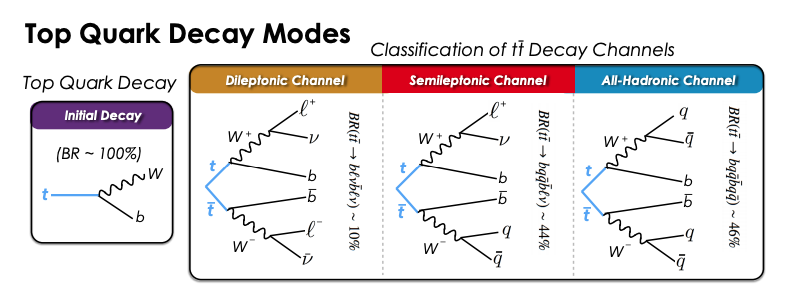
\includegraphics[width=0.8\linewidth]{Figures/ttbar-decay-mode.png}
	\caption{The schematic of Top quark decay channels.\cite{Mccarthy:2015ucy}}
	\label{fig:ttbardecaymode}
\end{figure}
\section{Machine Learning and its application on Particle Physics}

Machine Learning has been applied to most of the region in recent age, so dose particle physics. From the search of higgs boson(neural network and BDT) to the b-tagging technology(BDT\cite{Paganini:2017dpd}), physicist already applied several kinds of machine learning method to recent researchs.
\\
In a nutshell, machine learning can break into several cases, it can help to do classification, regression, and clustering problems. It can not only help to accelerate the computation of well-defined problems, and also find a new path to unsolved area. We will use a state-of-the-art machine learning technology, attention mechanism. The attention mechanism is a technology base on the evolution of Recurrent Neural Networks(RNN).\cite{A.Vaswani:2017} The attention mechanism will not only consider the local relationship and the sequence neighbor but also calculate the global relation base on the self-attention calculation shown in Figure \ref{fig:attention}. Using this novel architecture, we will train on the relationship between each jet and try to figure out the correct pair information.
\\
\begin{figure}[h]
	\centering
	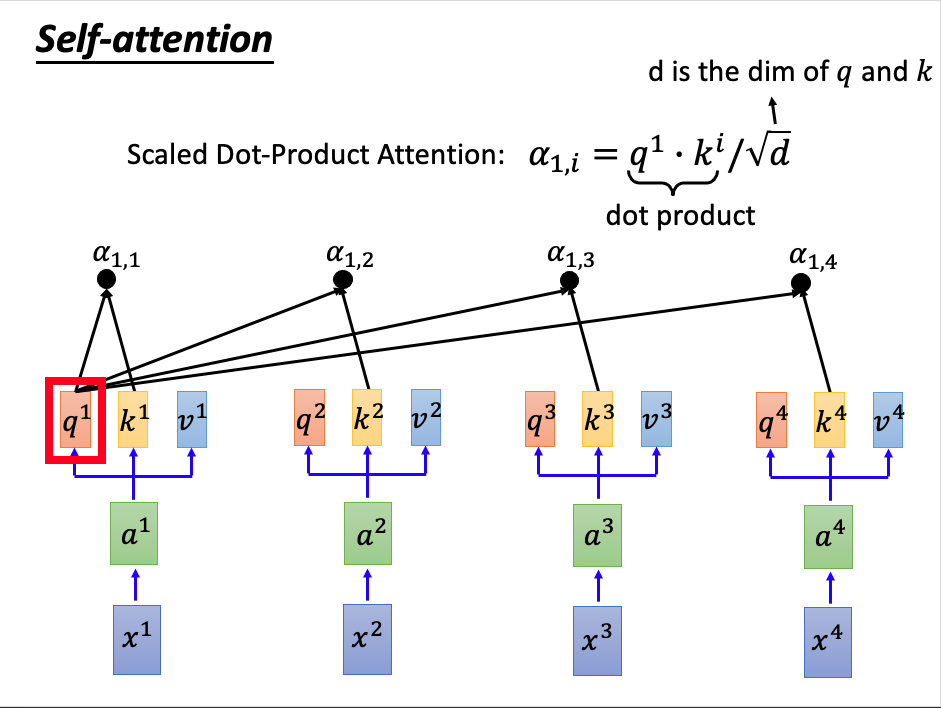
\includegraphics[width=0.8\linewidth]{Figures/attention.png}
	\caption{How self-attention works.\cite{HY.Lee:2019}}
	\label{fig:attention}
\end{figure}
